\documentclass[t]{beamer}

% Load general definitions
% Preamble file - general definitions, package loading, etc.

%=================================
% Load packages
\usepackage{amssymb,amsmath}
\usepackage{graphicx}
\usepackage{url}
\usepackage{tikz}
\usetikzlibrary{mindmap,trees,arrows}
\usepackage{fancyvrb}
\usepackage[english]{babel}
\usepackage[latin1]{inputenc}
\usepackage{subfigure}
\usepackage{times}
\usepackage[T1]{fontenc}
\usepackage{cancel}
\usepackage{color}
\usepackage{listings}

%=================================
% Set mode
\mode<presentation>
{
	\usetheme{Madrid}
	\usecolortheme{whale}
	\useoutertheme{infolines}
	\setbeamercovered{invisible}
}

% Get rid of nav bar
\beamertemplatenavigationsymbolsempty

% Insert frame number at bottom of the page.
\usefoottemplate{\hfil\tiny{\color{black!90}\insertframenumber}} 

%=================================
% Define new commands

\newcommand\Real{{\mathbb{R}}}
%\newcommand{\vi}{\vspace{0.6\baselineskip}}
%\newcommand{\goodgap}{\hspace{\subfigtopskip}\hspace{\subfigbottomskip}}


% Equation environments
\newcommand{\beq}{\begin{equation}}
\newcommand{\eq}{\end{equation}}
\newcommand{\beqs}{\begin{equation*}}
\newcommand{\eqs}{\end{equation*}}
\newcommand{\beqn}{\begin{eqnarray}}
\newcommand{\eqn}{\end{eqnarray}}

% Bold variables
\newcommand{\mbf}[1]{\ensuremath{\mathbf{#1}}}

% Itemization
\newcommand{\bitem}{\begin{itemize}}
\newcommand{\eitem}{\end{itemize}}
\newcommand{\spitem}{\vskip 1em\item}
\newcommand{\bitems}{\begin{itemize}\item}
\newcommand{\benums}{\begin{enumerate}\item}
\newcommand{\eenum}{\end{enumerate}}

% color blocks
\newenvironment{colorblock}[2]{%
\setbeamercolor{block title}{#2}
\begin{block}{#1}}{\end{block}}

% Vertical spacing
\newcommand{\vone}{\vskip 1em}
\newcommand{\vhalf}{\vskip .5em}

% Frame environments
\newenvironment{ftst}[3][t]{%
\begin{frame}{environment=ftst,#1}
\frametitle{#2}
\framesubtitle{#3}}{\end{frame}}

\newenvironment{ftstf}[2]{
\begin{frame}[fragile,environment=ftstf]
\frametitle{#1}
\framesubtitle{#2}}{\end{frame}}

% colors
\definecolor{MyGray}{rgb}{0.5,0.5,0.5}
\definecolor{MyDBGray}{rgb}{0.1,0.1,0.4}
\definecolor{darkgreen}{rgb}{0,0.4,0}
\definecolor{black}{rgb}{0,0,0}
\def\defn#1{{\color{red} #1}}

% Footnote
\renewcommand{\thefootnote}{\alph{footnote}}

% Relaxed footnotes
\newcommand{\lfr}[1]{\let\thefootnote\relax\footnote{\tiny #1}}

% Verbatim environment - using FANCYVRB package
\DefineVerbatimEnvironment%
{rcode}{Verbatim}
{fontsize=\scriptsize}

% Verbatim environment - using LISTINGS package
%\lstnewenvironment{rcode} {\lstset{	language = R,
%									basicstyle = \scriptsize\ttfamily,
%									showspaces = false,
%									showstringspaces = false,
%									showtabs = false,
%									keywordstyle = \color{black}\bfseries,
%									commentstyle = \color{darkgreen},
%									numbers = none,
%									otherkeywords={	<-,
%													ggplot,
%													geom_boxplot,
%													facet_grid,
%													shapiro.test,
%													fligner.test,
%													glht,
%													with},
%									deletekeywords={data,
%													model,
%													residuals,
%													c,
%													axis,
%													default,
%													labels,
%													qq.text}}}%
%{}


% Specific definitions
\title[]{Design and Analysis of Experiments}
\subtitle[]{08 - Testing Equivalence and Non-Inferiority}
\author[]{Felipe Campelo\\{\footnotesize http://orcslab.cpdee.ufmg.br/}}
\institute{Graduate Program in Electrical Engineering}
\date{\scriptsize Belo Horizonte\\April 2016}

\begin{document}

% cover page
\setbeamertemplate{footline}{}
\begin{frame}
\begin{flushright}

\includegraphics[width=.25\textwidth]{../figs/principal_completa3_ufmg}
\end{flushright}
  \titlepage
  \begin{tikzpicture}[remember picture,overlay]
  \node[anchor=south east,xshift=-5pt,yshift=122pt] at (current page.south east) {\tiny Version 2.11};
  \node[anchor=south west,yshift=0pt] at (current page.south west) {
\includegraphics[width=.15\textwidth]{../figs/by-nc-sa.png}};
  \end{tikzpicture}  
\end{frame}

%=====

% quotation page
  \begin{frame}[b]
		\frametitle{}
\begin{columns}[T]
\column{0.77\textwidth}
\flushright{\small ``\textit{
Science makes people reach selflessly for truth\\
and objectivity; it teaches people to accept reality,\\
with wonder and admiration, not to mention\\
the deep awe and joy that the natural order of things\\
brings to the true scientist.}''\\\vskip 1em
Lise Meitner\\1878 - 1968 \\Austrian Physicist}\\
\column{0.23\textwidth}
\begin{tikzpicture}[remember picture,overlay]
\node[anchor=south east,yshift=25pt,xshift=0pt] at (current page.south east)
{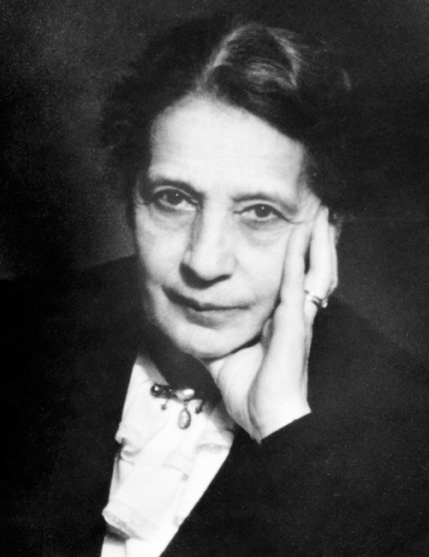
\includegraphics[width=\textwidth]{../figs/Meitner.jpg}};
\end{tikzpicture}
\end{columns}
\vhalf
\lfr{Image: \url{http://www.alltomvetenskap.se/nyheter/vem-var-86}}
\end{frame}

%=====
% Main slides

\begin{ftst}
{Testing equivalence}
{Introduction}
The tests introduced in the preceding chapters deal with situations in which one is interested in detecting \textit{differences} between a population parameter $\theta$ -- e.g., a population mean $\mu$ or a difference between population means $(\mu_1-\mu_2)$ -- and its nominal value $\theta_0$ under a null hypothesis;
\vone
Another useful class of experiments in engineering and science is one in which the experimenter is interesting in investigating \textit{equivalence} (within a given margin of error), for instance:

\bitems Conformity/compliance testing (industrial certification);
\spitem Equivalence of effects (pharmaceutical industry);
\eitem
\begin{tikzpicture}[remember picture,overlay]
\node[anchor=south east,yshift=5pt,xshift=-5pt] at (current page.south east)
{
\includegraphics[width=0.3\textwidth]{../figs/EquivDrugs.png}};
\end{tikzpicture}
\lfr{Image adapted from: \url{http://goo.gl/iXeCiY}}
\end{ftst}

%=====

\begin{ftst}
{Testing equivalence}
{Introduction}
In principle, one could express this as a shift in focus from trying to establish whether a population parameter is different from a given reference to trying to determine whether it is equal to that reference. 
\vone
In usual (two-sided) comparative studies, the alternative hypothesis (i.e., the one that presents novelty in relation to the current state of knowledge) is the one of difference between the parameters of interest - that is, unless there is strong evidence of differences, one cannot rule out the null hypothesis of equality;
\end{ftst}

%=====

\begin{ftst}
{Testing equivalence}
{Introduction}
In equivalence testing, the situation is reversed: the (approximate) equality of two parameters is the novelty one hopes to establish. Consequently, the burden of proof shifts to providing evidence that there is no difference.
\vone
The term \textit{equivalent} is not used strictly, but to mean the absence of practical differences - that is, any differences that might exist fall within an \textit{equivalence margin} or \textit{limit of practical significance} $\delta^*$.
\vone
Using this approach, the equivalence of two parameters can be established if a sample provides enough evidence that the true difference is smaller than $\delta^*$ units.
\end{ftst}

%=====

\begin{ftst}
{Testing Non-inferiority}
{Definition}
A similar concept to equivalence testing is the definition of non-inferiority of a given treatment/ process/ method in relation to another (e.g., a standard solution).
\vone
In non-inferiority tests, one can declare that a given process is not worse than a standard one only if enough evidence is provided to conclude that the performance of the proposed process is no more than $\delta^*$ units worse than that of the standard.
\vone
In the case of non-inferiority tests, one can in principle use a regular test of differences with a one-sided alternative (which would be equivalent to setting $\delta^* = 0$), or define the null hypothesis in a way that includes $\delta^*$ in its formulation.
\end{ftst}

%=====

\begin{ftst}
{Comparison of studies}
{\ }
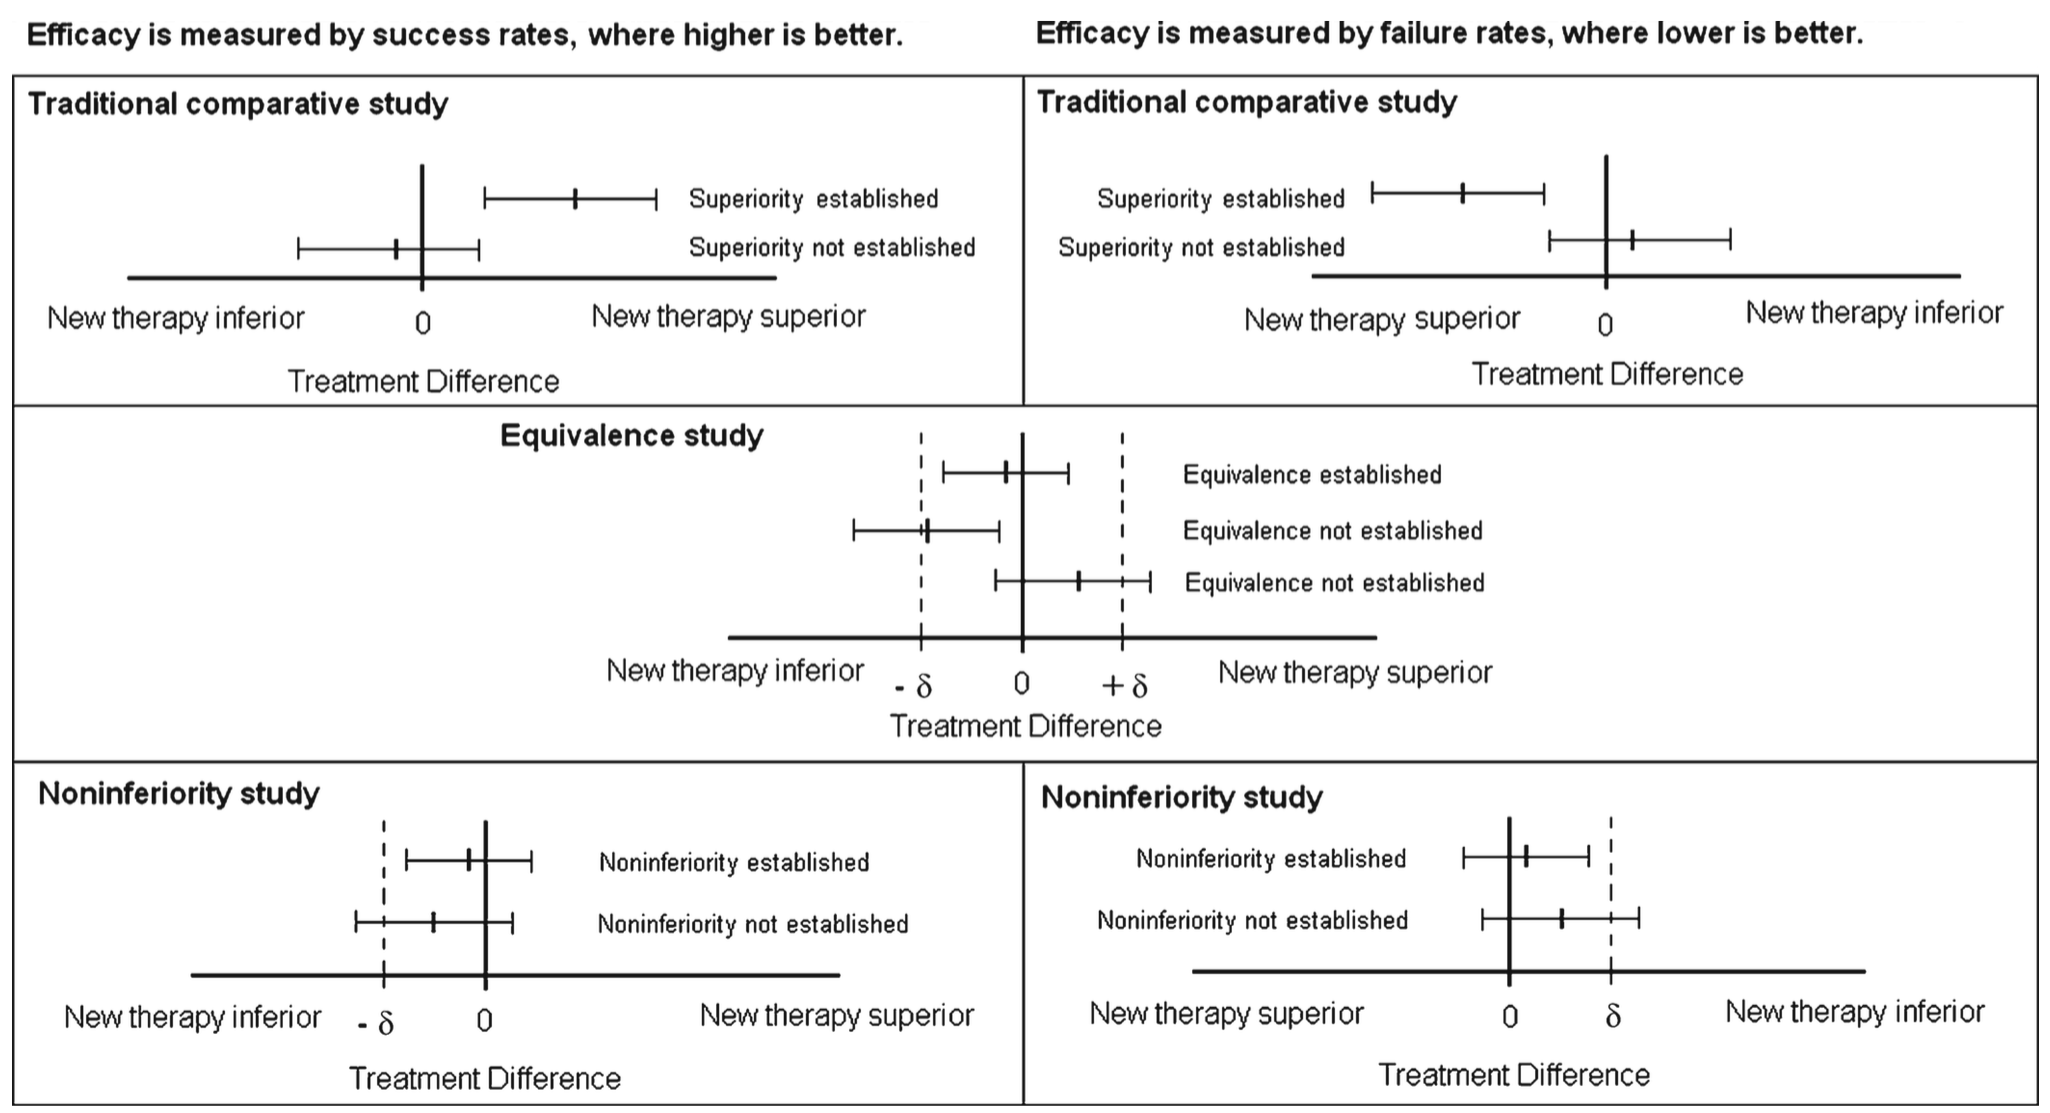
\includegraphics[width=\textwidth]{../figs/TOST.png}
\lfr{Image: Walker and Nowacki (2011), J. General Internal Medicine 26(2):192-196.}
\end{ftst}

%=====

\begin{ftst}
{Testing Equivalence}
{Quick-and-dirty approach}
A simple way of thinking about testing equivalence of two means is to observe confidence intervals instead of p-values:

\begin{colorblock}{}{bg=green,fg=black}
\centering ``\textit{Equivalence can be established at the $\alpha$ significance level if a $(1-2\alpha)$-confidence interval for the difference between the two means is contained within a interval $\pm\delta^*$.}''
\end{colorblock}

The difference between testing for differences and for equivalence can be easily illustrated using this approach:

\centering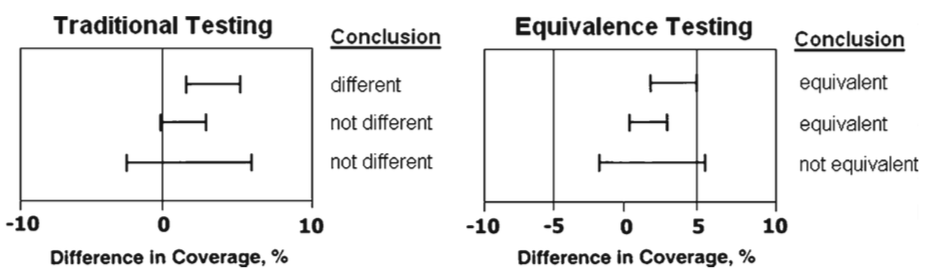
\includegraphics[width=.8\textwidth]{../figs/DiffVxEquiv.png}
\lfr{Image: Walker and Nowacki (2011), J. General Internal Medicine 26(2):192-196.}

\end{ftst}

%=====

\begin{ftst}
{Equivalence test for a single mean}
{Hypotheses}
An equivalence test for a single population mean can be expressed by the hypotheses:
\beqs
\begin{cases}
H_0: \left|\mu-\mu_0\right| = &\Delta\mu \geq\delta^*\\
H_1: &\Delta\mu <\delta^*
\end{cases}
\eqs
\vhalf
The most usual way of testing these hypotheses is the TOST (\textit{two one-sided tests}) method. As the name suggests, two one-sided significance tests are constructed so that the desired statistical properties can be achieved. Using our standard notation:
\begin{columns}[T]
\column{0.5\textwidth}
\beqs
\begin{cases}
H_0^1: &\Delta\mu = -\delta^*\\
H_1^1: &\Delta\mu > -\delta^*
\end{cases}
\eqs
\column{0.5\textwidth}
\beqs
\begin{cases}
H_0^2: &\Delta\mu = \delta^*\\
H_1^2: &\Delta\mu < \delta^*
\end{cases}
\eqs
\end{columns}
\vone
If both tests reject their respective $H_0$, then equivalence (within the equivalence margin $\delta^*$) can be declared with significance level $\alpha$.
\end{ftst}

%=====

\begin{ftst}
{Equivalence test for a single mean}
{Graphical interpretation}
\vskip 1em
\centering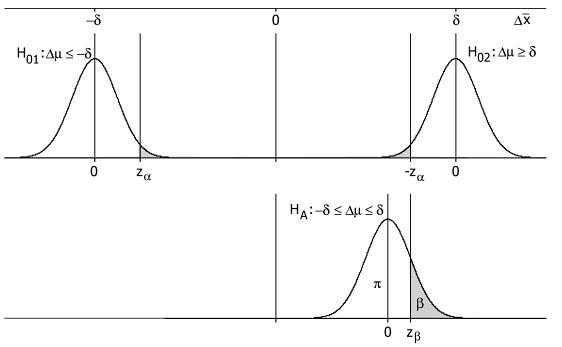
\includegraphics[width=.9\textwidth]{../figs/TOST-errors.png}
\lfr{Image: Matthews (2010), Sample Size Calculations, MMB. pg. 46}
\end{ftst}

%=====

\begin{ftst}
{Equivalence of a single mean}
{Sample size}
Sample sizes for testing equivalence of a single mean can be derived using essentially the same considerations used for the usual tests. In the case of a single sample:
\beqs
n\geq\left(\frac{\left(t_{\alpha}+t_{\beta}\right)\hat{\sigma}}{\delta^* - \Delta\mu}\right)^2
\eqs
\vone
As in the previous cases, iteration is needed to solve for $n$ (since the quantiles of the t distribution depend on $n$). Use $t_x$ = $z_x$ for the first iteration.
\end{ftst}

%=====

\begin{ftst}
{Equivalence of two means}
{Hypotheses}
Analogously to the single sample test of equivalence, the hypotheses for testing the equivalence of two population means can be described as:
\beqs
\begin{cases}
H_0: &\mu_1-\mu_2 \geq\delta^*\\
H_1: &\mu_1-\mu_2 <\delta^*
\end{cases}
\eqs
\hrulefill
\begin{columns}[T]
\column{0.5\textwidth}
\beqs
\begin{cases}
H_0^1: &\mu_1-\mu_2 = -\delta^*\\
H_1^1: &\mu_1-\mu_2 > -\delta^*
\end{cases}
\eqs
\column{0.5\textwidth}
\beqs
\begin{cases}
H_0^2: &\mu_1-\mu_2 = \delta^*\\
H_1^2: &\mu_1-\mu_2 < \delta^*
\end{cases}
\eqs
\end{columns}
\vone
Just as in the previous case, both hypotheses are tested at the desired $\alpha$ value, and the rejection of both $H_0$ indicates evidence of equivalence.
\end{ftst}

%=====

\begin{ftst}
{Equivalence of two means}
{Sample size}
Sample size for the $n_1 = n_2 = n$ case can be approximated based on the Zhang formula\footnote[1]{\tiny Zhang (2003), J. Biopharm. Stat. 13(3):529-538.}:
$$n \geq \left(t_{\alpha;\nu}+t_{(1-c)\beta;\nu}\right)^2\left(\frac{\hat{\sigma}_1^2+\hat{\sigma}_2^2}{\delta^*-\Delta\mu^*}\right)^2$$

\noindent with $\Delta\mu^*<\delta^*$ as the maximum real difference between the two means for which a power of $(1-\beta)$ is desired, and:
$$c = \frac{1}{2}\exp\left(-7.06\frac{\Delta\mu^*}{\delta^*}\right)$$

The degrees of freedom $\nu$ of the t-quantiles are given by the Welch t-test formula (see Chapter 6).
\end{ftst}

%=====

\begin{ftst}
{Example}
{Laboratory certification}
A ballistics laboratory is in the process of being\\
certified for the evaluation of shielding technology,\\
and needs to provide evidence of equivalence of a\\
given callibration procedure with the reference\\equipment;
\vone
The certification authority demands that the mean hole area generated by this procedure in the lab be the same as the one from the reference equipment, and tolerates deviations no greater than $4 mm^2$;
\vone
From previous measurements, the standard deviations can be roughly estimated as $\hat{\sigma}_{Lab} = 5 mm^2$ and $\hat{\sigma}_{ref} = 10 mm^2$.
\vone
The desired error levels for the comparison are $\alpha=0.01$ and $\beta = 0.1$.
\begin{tikzpicture}[remember picture,overlay]
\node[anchor=north east,yshift=-35pt,xshift=2pt] at (current page.north east) {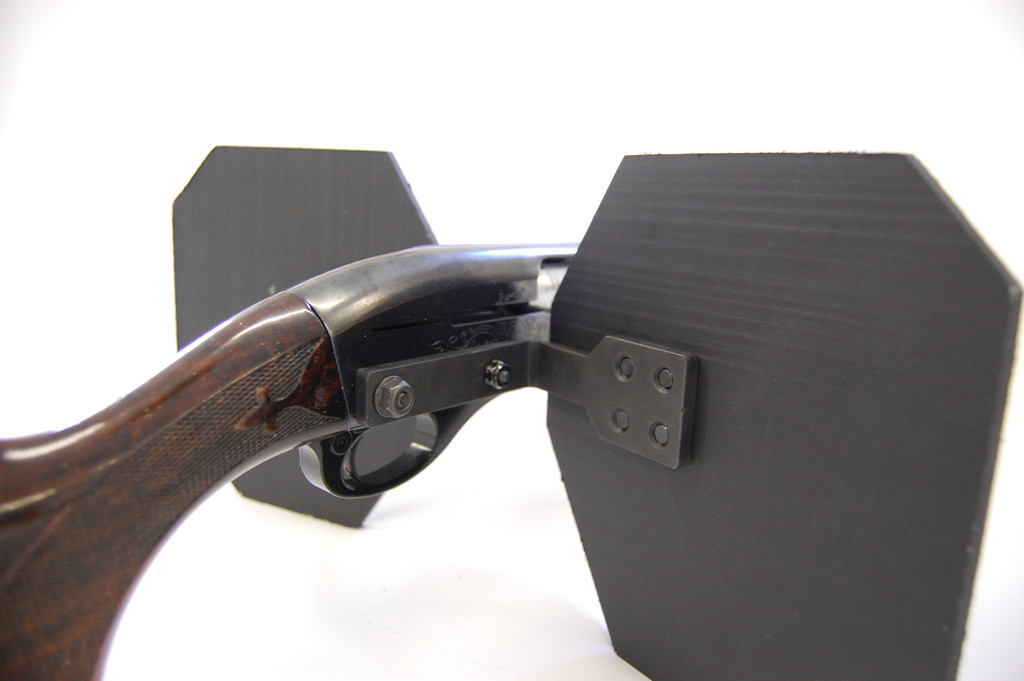
\includegraphics[width=.3\textwidth]{../figs/Shotgun-Ballistic-Shield.png}};
\end{tikzpicture}  

\lfr{Image: \url{http://www.everydaynodaysoff.com/2013/08/05/ballistic-shield-for-operators-only/}}
\end{ftst}

%=====

\begin{ftstf}
{Example}
{Laboratory certification}
To calculate the required sample size, assume that $\Delta\mu^* = 0.5$. Then:
\begin{rcode}
> # load functions to calculate sample size for TOST
> source("calcN_tost.R")
> 
> # Calculate sample size
> calcN_tost2(alpha = 0.01,
+             beta = 0.1,
+             diff_mu = 0.5,
+             tolmargin = 4,
+             s1 = 5,
+             s2 = 10)
[1] 144.1999
\end{rcode}
\vhalf
We'll need 145 observations from each group to test for equivalence with the desired experimental properties.
\end{ftstf}

%=====

\begin{ftstf}
{Example}
{Laboratory certification}
After collecting the observations, we proceed to the analysis:
\begin{rcode}
> data<-read.table("../data files/labdata-example.csv",
+                  header = T, sep = ",")

> # Two one-sided t-tests
> t.test(HoleArea~Place,  data = data,  alternative = "less", mu = 4,
+        conf.level = 0.99)$p.value
[1] 0.00304124
> t.test(HoleArea~Place, data = data, alternative = "greater", mu = -4,
+        conf.level = 0.99)$p.value
[1] 6.586193e-10

> # Get (1-2*alpha) CI 
> t.test(HoleArea~Place, data = data,  conf.level = 0.98)$conf.int
[1] -0.5117627  3.6244386
\end{rcode}
\begin{tikzpicture}[remember picture,overlay]
\node[anchor=south east,yshift=0pt,xshift=0pt] at (current page.south east) {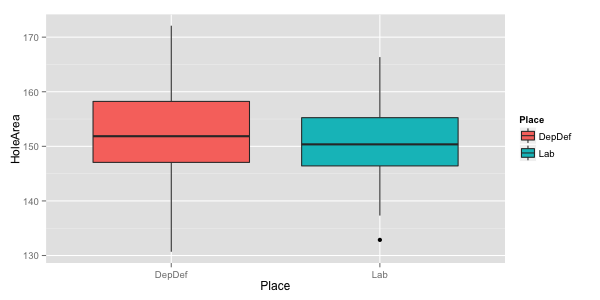
\includegraphics[width=.45\textwidth]{../figs/labdata.png}};
\end{tikzpicture}  
\end{ftstf}

%=====

\begin{ftstf}
{Example}
{Laboratory certification}
Verification of test assumptions:
\begin{rcode}
> par(mfrow=c(1,2))
> qqPlot(subset(data, Place=="Lab")[,2],
+        pch=20,
+        main = "Laboratory",
+        ylab = "Observed quantiles")
> qqPlot(subset(data, Place=="DepDef")[,2],
+        pch=20,
+        main = "Dept. Defence",
+        ylab = " ")
\end{rcode}
\begin{tikzpicture}[remember picture,overlay]
\node[anchor=south east,yshift=0pt,xshift=0pt] at (current page.south east) {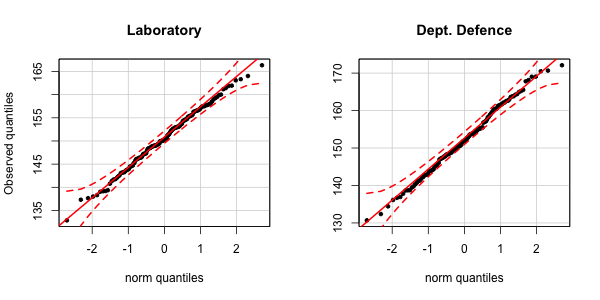
\includegraphics[width=.7\textwidth]{../figs/labdata-qqplots.png}};
\end{tikzpicture}  
\end{ftstf}

%=====

\begin{ftstf}
{Example}
{Laboratory certification}
Verification of test assumptions:
\begin{rcode}
> dwtest(HoleArea~Place, data=data)
DW = 1.8116, p-value = 0.04757

> par(mfrow=c(1,2))
> plot(seq_along(subset(data, Place=="Lab")[,2]),
+      subset(data, Place=="Lab")[,2], ...)
> plot(seq_along(subset(data, Place=="DepDef")[,2]),
+      subset(data, Place=="DepDef")[,2], ...)
\end{rcode}
\begin{tikzpicture}[remember picture,overlay]
\node[anchor=south east,yshift=0pt,xshift=0pt] at (current page.south east) {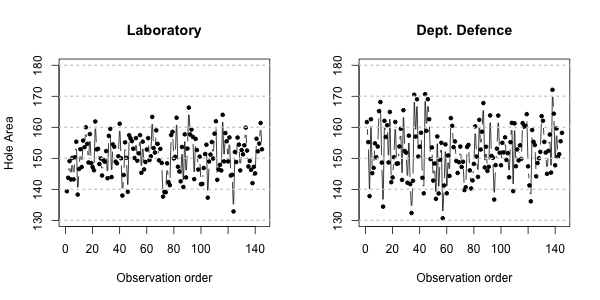
\includegraphics[width=.7\textwidth]{../figs/labdata-resplot.png}};
\end{tikzpicture}  
\end{ftstf}


%=====

\begin{ftst}
{Bibliography}
{\ }
\scriptsize
\textbf{Required reading}

\benums  E. Walker, A.S. Nowacki, \textit{Understanding Equivalence and Noninferiority Testing}, Journal of General Internal Medicine 26(2):192-196, 2011.
\eenum

\textbf{Recommended reading}

\benums P. Mathews, \textit{Sample Size Calculations: Practical Methods for Engineers and Scientists}, Ch. 2.4, 1st ed., MMB, 2010.
\item P. Zhang, \textit{A Simple Formula for Sample Size Calculation in Equivalence Studies}, Journal of Biopharmaceutical Statistics 13(3):529-538, 2003.
\eenum
\end{ftst}

%=====

\begin{ftstf}{About this material}{Conditions of use and referencing}
\centering\footnotesize This work is licensed under the Creative Commons CC BY-NC-SA 4.0 license\\(Attribution Non-Commercial Share Alike International License version 4.0).\\
\vhalf
\url{http://creativecommons.org/licenses/by-nc-sa/4.0/}\\
\vone
\footnotesize Please reference this work as:\\
\footnotesize \flushleft Felipe Campelo (2015), \textit{Lecture Notes on Design and Analysis of Experiments}.\\Online: {\scriptsize\url{https://github.com/fcampelo/Design-and-Analysis-of-Experiments}}\\
Version 2.11, Chapter 8; Creative Commons BY-NC-SA 4.0.\\

\begin{Verbatim}[fontsize=\tiny]
    @Misc{Campelo2015-01,
      title={Lecture Notes on Design and Analysis of Experiments},
      author={Felipe Campelo},
      howPublished={\url{https://github.com/fcampelo/Design-and-Analysis-of-Experiments}},
      year={2015},
      note={Version 2.11, Chapter 8; Creative Commons BY-NC-SA 4.0.},
    }
\end{Verbatim}

\begin{tikzpicture} [remember picture,overlay]
\node[anchor=south,yshift=0pt] at (current page.south){ \includegraphics[width=.2\textwidth]{../figs/CCSomerights.png}};
\end{tikzpicture}
\end{ftstf}


\end{document}